\subsection{The Topic/Problem}

The problem at hand involves the simulation of chemically reacting flows, the
governing equations of which amount to the Navier-Stokes equations with (in
our form):
\begin{itemize}
\item{A source term added to the energy equation in the form of heat flux}
\item{The addition of a governing equation for the rate of change of the
      mass fractions of each species in the chemical mechanism simulated}
\item{The addition of governing equations specifying the rate of change of
      temperature and pressure, derived from a constant internal energy
      assumption (for the former) and the ideal gas law (for the latter).}
\end{itemize}
These equations are given below, along with a brief explanation of the notation/nomenclature
used.
\begin{align}
\frac{\partial \rho}{\partial t} + \frac{\partial}{\partial x_{j}}(\rho u_{j}) &= 0 \\
\frac{\partial}{\partial t}(\rho u_{i}) + \frac{\partial}{\partial x_{j}}(\rho u_{i} u_{j} + P\delta_{ij} - \tau_{ij}) &= 0 \\
\frac{\partial}{\partial t}(\rho E) + \frac{\partial}{\partial x_{j}}((\rho E + P)u_{j} + q_{j} - u_{i}\tau_{ij}) &= 0 \\
\frac{\partial}{\partial t}(\rho Y_{k}) + \frac{\partial}{\partial x_{j}}(\rho Y_{k} u_{j} - \varphi_{ki}) &= W_{k}\dot{\omega}_{k} \\
\frac{\partial T}{\partial t} + \frac{\sum_{k=1}^{N_{sp}}U_{k}(T)\frac{\partial \rho Y_{k}}{\partial t}\frac{1}{W_{k}}}{\sum_{k=1}^{N_{sp}}[C]_{k}C_{v,k}(T)} &= 0 \\
\frac{\partial P}{\partial t} - \frac{R}{V}(T\frac{\partial n}{\partial t} + \frac{\partial T}{\partial t}n) &= 0
\end{align}
In these equations, $\rho$ is the fluid density, $u_{i}$ is the velocity in the $i$-th direction, and $E$ is the total energy.
$\delta_{ij}$ is the Kronecker delta, $P$ is the pressure, $T$ is the temperature, and $Y_{k}$ is the mass fraction of
species $k$. $[C]_{k}$ is the concentration of species $k$ in the gas mixture, $C_{v,k}(T)$ is the specific heat at constant volume
of species $k$ at temperature $T$, and $U_{k}(T)$ is the internal energy of species $k$ at temperature $T$. $N_{sp}$ is the number
of species in the chemical mechanism, $W_{k}$ is the molecular weight of species $k$, $n$ is the number of moles of the gas mixture,
V is the volume of the gas, and $\dot{\omega}_{k}$ is the net production rate of species $k$. $\tau_{ij}$ is the viscous stress
tensor, $\varphi_{ki}$ are the diffusion fluxes, and $q_{j}$ are the heat fluxes, defined by
\begin{align}
q_{j} = - \frac{\partial (\lambda T)}{\partial x_{j}} + h_{k}\varphi_{kj}.
\end{align}
In this expression, $\lambda$ is the thermal conductivity, and $h_{k}$ is the enthalpy of species $k$.
As for the diffusion fluxes, these are defined using a mixture-averaged approach - that is, $\varphi_{ki}$
is given by
\begin{align}
\varphi_{ki} = \varphi_{ki}^{*} + \varphi_{ki}^{c},
\end{align}
where $\varphi_{ki}^{*}$ is the mixture-averaged approximation, and $\varphi_{ki}^{c}$
is a correction term to ensure mass conservation. The mixture-averaged approximation
is defined by
\begin{align}
\varphi_{ki}^{*} = -\rho D_{k,m}\frac{W_{k}}{W} \frac{\partial X_{k}}{\partial x_{i}}
\end{align}
where $D_{k,m}$ is the mixture-averaged diffusivity of species $k$, $W$ is the mean
molecular weight, and $X_{k}$ is the mole fraction of species $k$. Finally, the
correction term is given by
\begin{align}
\varphi_{ki}^{c} = -Y_{k} \sum_{n=1}^{N_{sp}} \varphi_{ni}^{*}
\end{align}

In this set of governing equations (1) - (6), the mass fraction source term
on the right side of equation (4) is typically observed to be stiff relative
to the surrounding equations governing the motion of the gas mixture and the change
in its physical properties. This presents a time integration problem in that this term
alone typically dictates either an oppressively low timestep or the need for
an implicit approach, often using tools such as CVODE. In practice, fluid solvers
also often decouple an explicit treatment of the Navier-Stokes equations (1) - (3)
from the implicit treatment of the chemical kinetics, resulting in a splitting
approach that is at best first order in time.

The topic of this section of the proposal, then, is to answer the following
research question: \textbf{can we derive performance and/or temporal accuracy benefits
from an application of multi-rate Adams integrators to this set of governing
equations?}

%===========================================================================
\subsection{Goals and Bounds}

For outlining purposes, we will parse this section into a set of "must-haves",
"nice-to-haves", and aspects of the problem described above that are deemed
beyond the bounds of an eventual PhD thesis.

\subsubsection{Must-Haves}

The most obvious must-have is a demonstration of a novel time integration
scheme driving a canonical or especially demonstrative reacting flow problem
(ideally one that points directly to real-world impact) with improved efficacy
identified by either superior accuracy/stability or faster performance. Also
critical in this effort will be maintaining a solution that lies on the ideal
gas constraint manifold (i.e. a physical solution) - this has been identified
in early work as a potential sticking point when fully differential approaches
to solving the governing equations (as opposed to differential-algebraic approaches
that directly satisfy the constraints) are used. While the currently working
method of solving the equations uses a chemical kinetic Jacobian modified
to include the algebraic constraints explicitly, fully differential approaches
that use attenuation to force the solution towards the constraint manifold may
also be employed to greater effect.

\subsubsection{Nice-to-Haves}

Perhaps most prominent among the nice-to-haves is a thorough investigation of
the design space presented by the multi-rate framework we will use for time
integration (see \emph{The Plan}). The design choices inherent to this
scheme include:
\begin{itemize}
\item{Evaluation order ("fastest-first" vs. "slowest-first")}
\item{Re-extrapolation}
\item{Inclusion of additional history beyond order requirements (shown in \cite{mikida2019multi} to provide real-axis stability improvement)}
\item{Which solution components to include in error estimation for adaptive timestep
      control}
\item{Whether error control is accomplished through timestep control or step ratio control}
\end{itemize}
Another nice-to-have would amount to comparison of our scheme with CVODE as
a proxy for the state of the art in time integration of chemically reacting
flows, ideally achieving superiority in terms of observed temporal accuracy
of the entire system, or in terms of performance (most accurately measurable
by a reduction in the number of chemistry right-hand-side evaluations required
to reach a given solution time).

\subsubsection{Beyond Our Bounds}

An aspect of the algorithms being implemented that has been identified early
as beyond our bounds is the presence of multi-variable solves in a number of
potential adaptive implicit integration scenarios, namely:
\begin{itemize}
\item{Coupled implicit right-hand-sides}
\item{Use of adaptive timestep controllers where the local error estimate
      of all solution components makes use of implicit and explicit state
      estimates.}
\end{itemize}

%===========================================================================
\subsection{The Plan}

\subsubsection{Numerics}

The general path forward is to implement multi-rate Adams integrators (demonstrated
in \cite{mikida2019multi} as being a viable vehicle for performance improvement) with
the added ability to not only integrate the chemistry right-hand side implicitly, but
also to adapt the timestep of the resulting multi-rate integrator based on relative and/or
absolute local error demands. This latter capability would serve to match a similar
capability provided by CVODE while also maintaining the coupling between the fluid and the
chemistry (as well as the timestep flexibility) provided by the multi-rate framework.

In its current form, the timestep control algorithm used is that of ODE45, wherein
a timestep multiplier $r$ is calculated based on a local error estimate constructed from
state estimates of two (differing) explicit orders:
\begin{align}
r = \frac{\|s_{q+1} - s_{q}\|_{2}}{\text{ATOL} + \text{RTOL} \cdot \text{max}(\|s_{q}\|_{2}, \|s_{q+1}\|_{2})}
\end{align}
Here, $s_{q}$ is the state estimate obtained using an order-$q$ scheme, and ATOL and RTOL are absolute and
relative error tolerances specified by the user. Once $r$ is calculated, the timestep is \emph{decreased} if
$r>=1$ via
\begin{align}
\Delta t = 0.9\Delta t (r)^{-1/q}
\end{align}
and \emph{increased} if $r<1$ via
\begin{align}
\Delta t = 0.9\Delta t (r)^{-1/(q+1)}
\end{align}

As mentioned in the previous section of this outline, this added capability alone
presents a number of questions in terms of how best to accomplish this error control.
In particular, step ratio adjustment in situ, rather than timestep adjustment, to meet
error needs provides an implementation challenge in terms of code generation of these
integrators, whereas the choice of which solution component(s) are involved in
error estimation/timestep control also presents a design decision that could have
notable effect on numerical performance.

\subsubsection{Test Problem: Reacting Crossflow}

With the plan for the numerical methods to be implemented in place, the dominant
planning question then becomes: what is the test problem to which these new methods will
be applied to establish their viability? The current plan is to use a reacting mixing layer
problem with a hyperbolic tangent velocity profile for the baseflow (as used by \cite{michalke1964inviscid}
and \cite{blumen1970shear}), with the San-Diego 9-species chemical mechanism employed for
the chemical kinetics. By perturbing this baseflow with the mode having the highest growth
rate to instability (based on the inviscid analyses of \cite{michalke1964inviscid} and
\cite{blumen1970shear}), we can establish a fast-evolving solution component (the chemical
kinetics/mass fractions of the species) and a slow-evolving solution component (the fluid),
both possessing accessible means of rate modification (for the chemistry, we can accomplish
this by scaling the pre-exponential factors in the Arrhenius reaction rates, and for the
fluid, we can scale the magnitude of the initial crossflow).

\begin{figure}
\centering
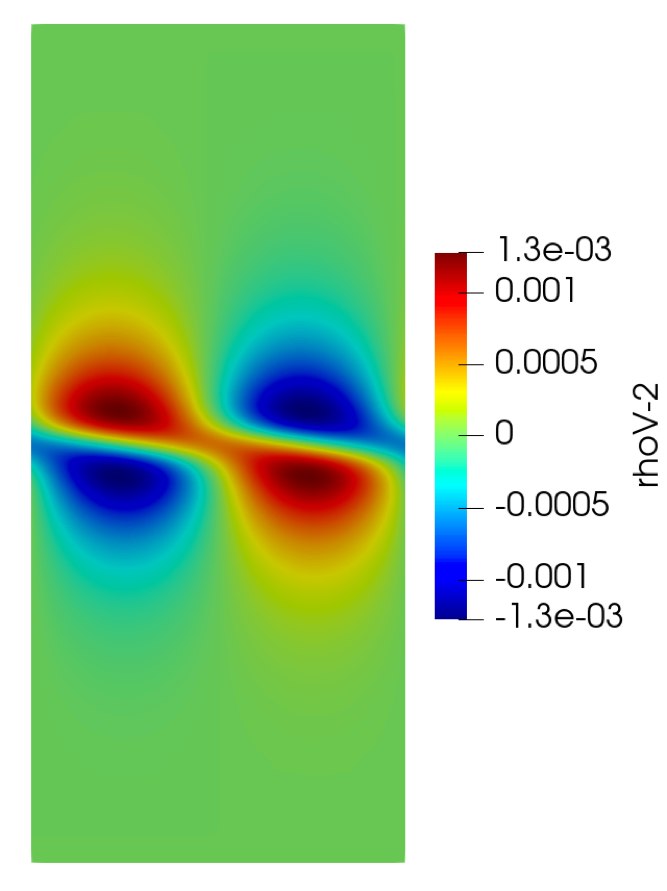
\includegraphics[width=0.3\linewidth,trim=4 4 4 4,clip]{figures/hyperbolic_tangent.png}
\caption{Perturbed vertical momentum of the hyperbolic tangent example - multispecies cold flow.}
\label{fig:hyperbolic_cold_rhov2}
\end{figure}

In doing so, what should result is a problem with ample testbed capabilities for our
new multi-rate integrators, and also a problem firmly rooted in physical utility in that
it provides the simplest model for scramjet/ramjet combustion.

%===========================================================================
\subsection{Impact}

The proposed thesis has the potential to have a significant impact on the
simulation of reacting flows, of which there are countless real-world applications
including (but not limited to) subsonic and supersonic combustion for propulsion
(gas turbines, ramjets/scramjets, rockets), furnaces and residential heating, and
solution of problems relating to atmospheric sciences.

The proposed work would also serve to augment the capabilities of Leap and Dagrt,
two Python packages for code generation of time integrators, by implementing the
proposed integrators. While this work would focus the attention of those new
integrators on reacting flows, additional useful application of implicit-explicit multi-rate
with error-based step control amongst the software's user base is possible, if not
probable.

Finally, the proposed work would also formally introduce new capabilities
to another existing combustion software package, PyJac-V2. This software is
responsible for code generation of callable source term and Jacobian functions
for chemical kinetics, and our work (given its application to problems that
often have large temperature ranges, not to mention a focus on high accuracy)
would add a NASA9 polynomial representation of thermodynamic quantities to
its codebase.

%===========================================================================
\subsection{Risk Mitigation}

An important question to ask amidst all of these promises is: 
textbf{what if this doesn't work out?} Assuming demonstration of improved
performance or accuracy of the \emph{multi-rate} integrators over the
state-of-the-art is for reasons unforseen impossible, a "fallback" takeaway
would be demonstration of improvement over the CVODE-fluid first-order splitting
approach via Leap implementation of an existing IMEX Runge-Kutta based scheme
that treats the chemistry implicitly via code-generated analytical Jacobians.
Given the use of a coupled implicit-explicit scheme (for which high order has
already been proven in other circumstances), as well as a chemical Jacobian
that is more accurately obtained than via finite differences (the method
of CVODE), this outcome should be attainable at minimum.

%===========================================================================
\subsection{Current Status}

At present, implicit-explicit time integration of reacting flows using Runge-Kutta
based methods in conjunction with code generation of source terms and Jacobians for
the chemical mechanisms is implemented and undergoing testing with the fluid solver
application. Implicit Adams methods (with single-rate Adams-Moulton being the baseline)
for the purposes of chemistry integration are also being implemented, along with
an application of the error-informed timestep control algorithm to both
single-rate and multi-rate Adams methods. Construction of implicit-explicit multi-rate
Adams methods with error-informed adaptivity are well underway, with testing
of these new methods on small-scale Cantera reactor system problems in progress.

As for the reacting crossflow validation problem, an initial setup employing
cold flow (no autoignition) with the perturbed baseflow applied to a nine-species
(San Diego) gas mixture is complete, with validation via the growth rate of the
unstable mode ongoing. Also implemented in the reacting flow solver is a one-dimensional
laminar free flame problem, which may also be used as a first-pass validation (via comparison
to the Cantera-estimated steady-state flame speed) for new integration methods for reacting
flows as they become available.

%===========================================================================
